% !TEX root = ../../document.tex

\documentclass{subfiles}

\begin{document}

  \chapter{Estructuras de Datos de Resumen}
  \label{chapter:summaries}

    \section{Introducción}
    \label{sec:summaries_intro}

      \paragraph{}
      El gran crecimiento tecnológico que se está llevando a cabo en la actualidad a todos los niveles está propiciando además un aumento exponencial en cuanto a la cantidad de información que se genera. La reducción de costes en cuanto a la instalación de sensores que permiten recoger información de muchos procesos productivos, así como la obtenición de metadatos a partir del uso de internet y las redes sociales por parte de los usuarios hace que el ritmo de crecimiento en cuanto a cantidad información generada por unidad de tiempo haya crecido a un ritmo frenético.

      \paragraph{}
      Una de las razones que han facilitado dicha tendencia es la disminución de costes de almacenamiento de información, a la vez que han aumentado las capacidades de cómputo necesarias para procesarla. Sin embargo, debido al crecimiento exponencial de los conjuntos de datos, es necesario investigar nuevas técnicas y estrategias que permitan obtener respuestas satisfactorias basadas en la gran cantidad de información de la que se dispone en un tiempo razonable.

      \paragraph{}
      Tradicionalmente, la investigación en el campo de las \emph{bases de datos} se ha centrado en obtener respuestas exactas a distintas consultas, tratando de hacerlo de la manera más eficiente posible, así como de tratar de reducir el espacio necesario para almacenar la información. \emph{Acharya y otros} proponen en el artículo \emph{Join synopses for approximate query answering} \cite{acharya1999join} el concepto de \emph{Approximate Query Processing}. Dicha idea se expone en la subsección \ref{sec:aproximate_query_processing}.

      \subsection{Approximate Query Processing}
      \label{sec:aproximate_query_processing}

        \paragraph{}
        El \emph{procesamiento de consultas aproximado}, (\emph{Approximate Query Processing} o \textbf{AQP}) se presenta como una estrategia de resolución de consultas basada en conceptos y propiedades estadísticas que permiten una gran reducción en la complejidad computacional y espacial necesaria para la resolución de las mismas por una base de datos. Por contra, dicha reducción a tiene como consecuencia la adicción de un determinado nivel de imprecisión en los resultados a la cual se denomina error. Se pretende que dicho error pueda ser acotada en un intervalo centrado en el valor verdadero con una desviación máxima determinada por $\epsilon$, y que la pertenencia de la solución a este intervalo se cumpla con una probabilidad $\delta$. Al igual que en el anterior capítulo, en este caso también se presta especial importancia a la minimización del error relativo, lo cual consigue que las soluciones mediante el \emph{procesamiento de consultas aproximado} sean válidas tanto para consultas de tamaño reducido como de gran tamaño.


      \paragraph{}
      Durante el resto del capítulo se describen y analizan distintas estrategias que permiten llevar a cabo implementaciones basadas en \emph{procesamiento de consultas aproximado} centrando especial atención en los \emph{Sketches} por su cercanía respecto del \emph{Modelo en Streaming} descrito en el capítulo \ref{chapter:streaming}. En la sección \ref{sec:summaries_types} se realiza una descripción a partir de la cual se pretende aclarar las diferencias entre las distintas estrategias de sumarización de grandes conjuntos de datos. Las estrategias que se describen son \emph{muestreo probabilístico}, mantenimiento de un \emph{histograma}, utilización de \emph{wavelets} y por último se describen en profundidad conceptos referidos a \emph{Sketches}. En las secciones \ref{sec:bloom_filter}, \ref{sec:count_min_sketch}, \ref{sec:count_sketch}, \ref{sec:ams_sketch} y \ref{sec:hyper_log_log} se habla del \emph{Bloom-Filter} \emph{Count-Min Sketch}, \emph{Count Sketch}, \emph{AMS Sketch} e \emph{HyperLogLog} respectivamente.


    \section{Tipos de Estructuras de Datos de Resumen}
    \label{sec:summaries_types}

      \paragraph{}
      Para el diseño de soluciones basadas en \emph{procesamiento de consultas aproximado} existen distintas estrategias, cada una de las cuales presentan ventajas e inconvenientes por lo que cada una de ellas es más conveniente para una determinada tarea, sin embargo en ocasiones surgen solapamientos entre ellas tal y como se pretende mostrar en esta sección. Dichas descripciones han sido extraidas del libro \emph{Synopses for massive data} \cite{cormode2012synopses} redactado por \emph{Cormode y otros}. En las secciones \ref{sec:sampling}, \ref{sec:histogram}, \ref{sec:wavelet} y \ref{sec:sketch} se habla de \emph{Sampling}, \emph{Histogram}, \emph{Wavelet} y \emph{Sketches} respectivamente.

      \subsection{Sampling}
      \label{sec:sampling}

        \paragraph{}
        El \emph{Sampling} o \emph{muestreo probabilístico} es la estrategia más consolidada de entre las que se presentan. Las razones se deben a su simplicidad conceptual así como su extendido uso en el mundo de la estadística. Uno de los primeros artículos en que se trata el muestreo aplicado a bases de datos es \emph{Accurate estimation of the number of tuples satisfying a condition} \cite{piatetsky1984accurate} redactado por \emph{Piatetsky-Shapiro} y \emph{Connell}. La intuición en que se basa esta solución es la selección de un subconjunto de elementos denominado \emph{muestra} extraida del conjunto global al cual se denomina \emph{población}. Una vez obtenida la \emph{muestra} del conjunto de datos global, cuyo tamaño es significativamente menor respecto del global (lo cual reduce drásticamente el coste computacional), se realizan los cálculos que se pretendía realizar sobre toda la \emph{población} para después obtener un estimador del valor real que habría sido calculado al realizar los cálculos sobre el conjunto de datos global.

        \paragraph{}
        Para que las estrategias de sumarización de información obtengan resultados válidos o significativos respecto del conjunto de datos, es necesario que se escojan adecuadamente las instancias de la \emph{muestra}, de manera que se maximice la similitud del resultado respecto del que se habría obtenido sobre toda la población. Para llevar a cabo dicha labor existen distintas estrategias, desde las más simples basadas en la selección aleatoria sin reemplazamiento como otras mucho más sofisticadas basadas en el mantenimiento de \emph{muestras} estratificadas. Sea $R$ la población y $|R|$ el tamaño de la misma. Denominaremos $t_j$ al valor $j$-ésimo de la población y $X_j$ al número de ocurrencias del mismo en la \emph{muestra}. A continuación se describen distintas técnicas de muestreo:

        \begin{itemize}

          \item \textbf{Selección Aleatoria Sin Reemplazamiento}: Consiste en la estrategia más simple de generación de \emph{muestras}. Se basa en la selección aleatoria de un valor entero $r$ en el rango $[1, |R|]$ para después añadir el elemento localizado en la posición $r$ de la \emph{población} al subconjunto de la \emph{muestra}. Este proceso se repite durante $n$ veces para generar una \emph{muestra} de tamaño $n$. A modo de ejemplo se muestra el estimador para la operación \emph{SUMA} en la ecuación \eqref{eq:sum_with_replacement}, además se muestra la fórmula de la desviación para dicho estimador en la ecuación \eqref{eq:sum_with_replacement_deviation}.
            \begin{align}
            \label{eq:sum_with_replacement}
              Y &= \frac{|R|}{n}\sum_jX_jt_j \\
            \label{eq:sum_with_replacement_deviation}
              \sigma^2(Y) &= \frac{|R|^2\sigma^2(R)}{n}
            \end{align}

          \item \textbf{Selección Aleatoria Con Reemplazamiento}: En este caso se supone que la selección de una instancia de la población tan solo se puede llevar a cabo una única vez, por lo tanto se cumple que $\forall X_j \in {0,1}$. La selección se lleva a cabo de la siguiente manera: se genera de manera aleatoria un valor entero $r$ en el rango $[1, |R|]$ para después añadir el elemento localizado en la posición $r$ de la \emph{población} al subconjunto de \emph{muestra} si este no ha sido añadido ya, sino volver a generar otro valor $r$. Después repetir dicha secuencia durante $n$ veces para generar una \emph{muestra} de tamaño $n$. Al igual que en la estrategia anterior, en este caso también se muestra el estimador para la operación \emph{SUMA} en la ecuación \eqref{eq:sum_without_replacement}. Nótese que el cálculo es el mismo que en el caso de la estrategia sin reemplazamiento. Sin embargo, la varianza obtenida a partir de dicha estrategia es menor tal y como se muestra en la ecuación \eqref{eq:sum_without_replacement_deviation}.
            \begin{align}
            \label{eq:sum_without_replacement}
              Y &= \frac{|R|}{n}\sum_jX_jt_j \\
            \label{eq:sum_without_replacement_deviation}
              \sigma^2(Y) &= \frac{|R|(|R| - n)\sigma^2(R)}{n}
            \end{align}

          \item \textbf{Bernoulli y Poisson}: Mediante esta alternativa de muestreo se sigue una estrategia completamente distinta a las anteriores. En lugar de seleccionar la siguiente instancia aleatoriamente de entre todas las posibles, se decide generar $|R|$ valores aleatorios $r_j$ independientes en el intervalo $[0,1]$ de tal manera que si $r_j$ es menor que un valor $p_j$ fijado a priori, la instancia se añade al conjunto de \emph{muestra}. Cuando se cumple que $\forall i, j \ p_i = p_j$ se dice que es un muestreo de \emph{Bernoulli}, mientras que cuando no se cumple dicha condición se habla de muestreo de \emph{Poisson}. El cálculo del estimador para la \emph{SUMA} en este caso es muy diferente de los ilustrados anteriormente tal y como se muestra en la ecuación \eqref{eq:sum_bernoulli_poisson}. La desviación de este estimador se muestra en la ecuación \eqref{eq:sum_bernoulli_poisson_deviation}, que en general presenta peores resultados (mayor desviación) que mediante otras alternativas, sin embargo, esta posee la cualidad de poder aplicar distintos pesos a cada instancia de la población, lo que puede traducirse en que una selección adecuada de los valores $p_j$, lo cual puede mejorar significativamente la precisión de los resultados si estos se escogen de manera adecuada.
            \begin{align}
            \label{eq:sum_bernoulli_poisson}
              Y &= \sum_{i \in muestra }\frac{t_i}{p_i} \\
            \label{eq:sum_bernoulli_poisson_deviation}
              \sigma^2(Y) &= \sum_i(\frac{1}{p_i}-1)t_i^2
            \end{align}

          \item \textbf{Muestreo Estratificado}: El muestreo estratificado trata de minimizar al máximo las diferencias entre la distribución del conjunto de datos de la \emph{población} respecto de la \emph{muestra} que se pretende generar. Para ello existen distintas alternativas entre las que se encuentra una selección que  actualiza los pesos $p_j$ tras cada iteracción, lo que reduce drásticamente la desviación de la \emph{muestra}, sin embargo produce un elevado coste computacional para su generación. Por tanto, existen otras estrategia más intuitivas basada en la partición del conjunto de datos de la \emph{población} en subconjuntos disjuntos que poseen la cualidad de tener varianza mínima a los cuales se denomina \emph{estratos}. Posteriormente, se selecciona mediante cualquiera de los métodos descritos anteriormente una \emph{muestra} para cada \emph{estrato}, lo cual reduce en gran medida la desviación típica global del estimador.

        \end{itemize}

        \paragraph{}
        La estrategia de sumarización de información mediante \emph{muestreo} tiene como ventajas la independencia de la complejidad con respecto a la dimensionalidad de los datos (algo que como se ilustrará con en posteriores secciones no sucede con el resto de alternativas) además de su simplicidad conceptual. También existen cotas de error para las consultas, para las cuales no ofrece restricciones en cuanto al tipo de consulta (debido a que se realizan sobre un subconjunto con la misma estructura que el global). El muestre es apropiado para conocer información general acerca del conjunto de datos. Además, presenta la cualidad de permitir su modificación y adaptación en tiempo real, es decir, se pueden añadir o eliminar nuevas instancias de la muestra conforme se añaden o eliminan del conjunto de datos global.

        \paragraph{}
        Sin embargo, en entornos donde el ratio de addiciones/eliminaciones es muy elevado el coste computacional derivado del mantenimiento de la muestra puede hacerse poco escalable. El \emph{muestreo} es una buena alternativa para conjuntos de datos homogéneos, en los cuales la presencia de valores atípicos es irrelevante. Tampoco obtiene buenos resultados en consultas relacionadas con el conteo de elementos distintos. En las siguientes secciones se describen alternativas que resuelven de manera más satisfactoria estas dificultades y limitaciones.

      \subsection{Histogram}
      \label{sec:histogram}

        \paragraph{}
        Los \emph{histogramas} son estructuras de datos utilizadas para sumarizar grandes conjuntos de datos mediante el mantenimiento de tablas de frecuencias, por lo que tienen un enfoque completamente diferente al que siguen las estrategias de \emph{muestreo} de la sección anterior. En este caso, el concepto es similar a la visión estadística de los histogramas. Consiste en dividir el dominio de valores que pueden tomar las instancias del conjunto de datos en intervalos o contenedores disjuntos entre si de tal manera que se mantiene un conteo del número de instancias pertenecientes a cada partición.

        \paragraph{}
        Durante el resto de la sección se describen de manera resumida distintas estrategias de estimación del valor de las particiones, así como las distintas estrategias de particionamiento del conjunto de datos. Para llevar a cabo dicha tarea, a continuación se describe la notación que se ha seguido en esta sección: Sea $D$ el conjunto de datos e $i \in [1,M]$ cada una de las categorías que se presentan en el mismo. Denotaremos por $g(i)$ al número de ocurrencias de la categoría $i$. Para referirnos a cada uno de las particiones utilizaremos la notación $S_j$ para $j \in [1, B]$. Nótese por tanto que $M$ representa el cardinal de categorías distintas mientras que $B$ representa el cardinal de particiones utilizadas para \say{comprimir} los datos. La mejora de eficiencia en cuanto a espacio se consigue devido a la eleccion de $B \ll M$

        \paragraph{}
        Cuando se hablamos de \emph{esquemas de estimación} nos estamos refiriendo a la manera en que se almacena o trata el contenido de cada una de las particiones $S_j$ del histograma. La razón por la cual este es un factor importante a la hora de caracterizar un histograma es debida a que está altamente ligada a la precisión del mismo.

        \begin{itemize}

          \item \textbf{Esquema Uniforme}: Los esquemas que presuponen una distribución uniforme de las instancias dentro del contenedor se subdividen en dos categorías: \begin{enumerate*} [label=\itshape\alph*\upshape)]
        			\item \emph{continous-value asumption} que presupone que todas las categorías $i$ contenidas en la partición $S_j$ presentan el mismo valor para la función $g(i)$ y
        			\item \emph{uniform-spread asumption} que presupone que el número de ocurrencias de la partición $S_j$ se localiza distribuido uniformemente al igual que en el caso anterior, pero en este caso entre los elementos de un subconjunto $P_j$ generado iterando con un determinado desplazamiento $k$ sobre las categorías $i$ contenidas en $S_j$.
        		\end{enumerate*} El segundo enfoque presenta mejores resultados en el caso de consultas de cuantiles que se distribuyen sobre más de una partición $S_j$

          \item \textbf{Esquema Basado en Splines}: En la estrategia basada en splines se presupone que los valores se distribuyen conforme una determinada función lineal de la forma $y_j = a_jx_j + b_j$ en cada partición $S_j$ de tal manera que el conjunto total de datos $D$ puede verse como una función lineal a trozos y continua, es decir, los extremos de la función en cada partición coinciden con el anterior y el siguiente. Nótese que en este caso se ha descrito la estrategia suponiendo el uso de una función lineal, sin embargo esta puede extenderse a funciones no lineales.

          \item \textbf{Esquema Basado en Árboles}: Consiste en el almacenamiento de las frecuencias de cada partición $S_j$ en forma de árbol binario, lo cual permite seleccionar de manera apropiada el nivel del árbol que reduzca el número de operaciones necesarias para obtener la estimación del conteo de ocurrencias según el la amplitud del rango de valores de la consulta. La razón por la cual se escoje un árbol binario es debida a que se puede reducir en un orden de $2$ el espacio necesario para almacenar dichos valores manteniendo únicamente los de una de las ramas de cada sub-árbol. La razón de ello es debida a que se puede recalcular el valor de la otra mediante una resta sobre el valor almacenado en el nodo padre y la rama que si contiene el valor.

          \item \textbf{Esquema Heterogéneo}: El esquema heterogéneo se basa la intuición de que la distribución de frecuencias de cada una de las particiones $S_j$ no es uniforme y tiene peculiaridades propias, por lo tanto sigue un enfoque diferente en cada una de ellas tratanto de minimizar al máximo la tasa de error producida. Para ello existens distintas heurísticas basadas en distancias o teoría de la información entre otros.

        \end{itemize}


        \paragraph{}
        Una vez descritas distintas estrategias de estimación del valor de frecuencias de una determinada partición $S_j$, el siguiente paso para describir un \emph{histograma} es realizar una descripción acerca de las distintas formas de generación de las particiones o contenedores. Para tratar de ajustarse de manera más adecuada a la distribución de los datos se puede realizar un \emph{muestreo} a partir del cual se generan las particiones. A continuación se describen las técnicas más comunes para la elaboración de dicha tarea:

        \begin{itemize}

          \item \textbf{Particionamiento Heurístico}: Las estrategias de particionamiento heurístico se basan en el apoyo sobre distintas presuposiciones que en la práctica han demostrado comportamientos aceptables en cuanto al nivel de precisión que se obtiene en los resultados, sin embargo, no proporcionan ninguna garantía desde el punto de vista de la optimalidad. Su uso está ampliamente extendido debido al reducido coste computacional. Dentro de esta categoría las heurísticas más populares son las siguientes:
            \begin{itemize}

              \item \textbf{Equi-Width}: Consiste en la división del dominio de categorías $[1,M]$ en particiones equi-espaciadas unas de otras. Para dicha estrategia tan solo es necesario conocer \emph{a-priori} el rango del posible conjunto de valores. Es la solución con menor coste computacional, a pesar de ello sus resultados desde el punto de vista práctico son similares a otras estrategias más sofisticadas cuando la distribución de frecuencias es uniforme.

              \item \textbf{Equi-Depth}: Esta estrategia de particionamiento requiere conocer la distribución de frecuencias \emph{a-priori} (o una aproximación que puede ser obtenida mediante alguna estrategia como el muestreo). Se basa en la división del dominio de valores de tal manera que las particiones tengan la misma frecuencia. Para ello se crean particiones de tamaños diferentes.

              \item \textbf{Singleton-Bucket}: Para tratar de mejorar la precisión esta estrategia de particionamiento se basa en la utilización de dos particiones especiales, las cuales contienen las categorías de mayor y menor frecuencia respectivamente para después cubrir el resto de categorías restante mediante otra estrategia (generalmente \emph{equi-depth}) lo cual se basa en la idea de que estas particiones especiales contendrán los valores atípicos y el resto de la muestra será más uniforme.

              \item \textbf{Maxdiff}: En este caso, el método de particionamiento se basa en la idea de utilizar los puntos de mayor variación de frecuencias mediante la medida $|g(i+1) - g(i)|$, para dividir el conjunto de categorías en sus respectivas particiones, de tal manera que las frecuencias contenidas en cada partición sean lo más homogéneas posibles entre sí.

            \end{itemize}
          \item \textbf{Particionamiento con Garantías de Optimalidad}: En esta categoría se enmarcan las estrategias de generación de particiones que ofrecen garantías de optimalidad a nivel de la precisión de resultados en las consultas. Para ello se utilizan técnicas de \emph{Programación Dinámica} (DP), de tal manera que la selección de las particiones se presenta como un problema de \emph{Optimización}. Sin embargo, dichas estrategias conllevan un elevado coste computacional que muchas veces no es admisible debido al gran tamaño del conjunto de datos que se pretende sumarizar. Como solución ante dicha problemática se han propuesto distintas estrategias que se basan en la resolución del problema de optimización, pero sobre una \emph{muestra} del conjunto de datos global, lo cual anula las garantías de optimalidad pero puede ser una buena aproximación si la muestra seleccionada es altamente representativa respecto de la población.

          \item \textbf{Particionamiento Jerárquico}: Las estrategias de particionamiento jerárquico se basan en la utilización de particiones siguiendo la idea de utilizar un árbol binario. Por lo tanto, las particiones no son disjuntas entre ellas, sino que se contienen unas a otras. Esto sigue la misma idea que se describió en el apartado de \emph{Esquemas de estimación Basados en Árboles}. Apoyandose en esta estrategia de particionamiento se consigue que las consultas de rangos de frecuencias tengan un coste computacional menor en promedio (aún en el casos en que el rango sea muy amplio). En esta categoría destacan los histogramas \emph{nLT} (n-level Tree) y \emph{Lattice Histograms}. Estos últimos tratan de aprovechar las ventajas a nivel de flexibilidad y precisión que presentan los histogramas, además de las estrategias jerárquicas de sumarización en que se apoyan las \emph{Wavelets} tal y como se describe en la siguiente sección.

        \end{itemize}

        \paragraph{}
        Las ideas descritas en esta sección sobre los \emph{histogramas} son extrapolables conforme se incrementa la dimensionalidad de los datos. En el caso de los esquemas de estimación, esto sucede de manera directa. Sin embargo, en el caso de los esquemas de particionamiento surgen distintos problemas debido al crecimiento exponencial tanto a nivel de espacio como de tiempo conforme aumenta el número de dimensiones de los datos por lo cual se convierten en soluciones impracticables para conjuntos de datos con elevada dimensionalidad

        \paragraph{}
        Los \emph{Histogramas} representan una estrategia sencilla, tanto a nivel de construcción como de consulta, la cual ofrece buenos resultados en un gran número de casos. Dichas estructuras han sido ampliamente probadas para aproximación de consultas relacionadas con suma de rangos o frecuencias puntuales. Tal y como se ha dicho previamente, su comportamiento en el caso unidimensional ha sido ampliamente estudiado, sin embargo, debido al crecimiento exponencial a nivel de complejidad conforme las dimensiones del conjunto de datos aumentan estas estrategias son descartadas en muchas ocasiones. Los \emph{Histogramas} requieren de un conjunto de parámetros fijados \emph{a-priori}, los cuales afectan en gran medida al grado de precisión de los resultados (pero cuando se seleccionan de manera adecuada esta solución goza de una gran cercanía al punto de optimalidad), por tanto, en casos en que la estimación de dichos valores necesarios \emph{a-priori} se convierte en una labor complicada, existen otras técnicas que ofrecen mejores resultados.

      \subsection{Wavelet}
      \label{sec:wavelet}

        \paragraph{}
        Las estructuras de sumarización denominadas \emph{Wavelets}, a diferencia de las anteriores, han comenzado a utilizarse en el campo del \emph{procesamiento de consultas aproximado} desde hace relativamente poco tiempo, por lo que su uso no está completamente asentado en soluciones comerciales sino que todavía están en fase de descubrimiento e investigación. Las \emph{Wavelets} (u \emph{ondículas}) se apoyan en la idea de representar la tabla de frecuencias del conjunto de datos como una función de ondas discreta. Para ello, se almacenan distintos valores (dependiendo del tipo de \emph{Wavelet}) que permiten reconstruir la tabla de frecuencias tal y como se describirá a continuación cuando se hable de la \emph{transformada de Haar}, la mejora de eficiencia en cuanto a espacio a partir de esta estructura de sumarización se basa en el mantenimiento aproximado de los valores que permiten reconstruir el conjunto de datos.

        \paragraph{}
        A continuación se describe la \emph{transformada de Haar}, a partir de la cual se presentan las distintas ideas en que se apoyan este tipo de estructuras de sumarización. En los últimos años se ha trabajado en estrategias más complejas como la \emph{Daubechies Wavelet} \cite{akansu2001multiresolution} de \emph{Akansu y otros} o la \emph{transformada de Wavelet basada en árboles duales completos} \cite{selesnick2005dual} de \emph{Selesnick y otros}.

        \subsubsection{Haar Wavelet Transform}

          \paragraph{}
          La \emph{Haar Wavelet Transform} (\textbf{HWT}) consiste en una construcción de carácter jerárquico que colapsa las frecuencias de las distintas categorías de manera pareada recursivamente hasta llegar a un único elemento. Por tanto, la idea es la similar a la creación de un árbol binario desde las hojas hasta la raiz. Esta estrategia es similar a la que siguen los \emph{Histogramas jerárquicos} de la sección anterior. Además, se aprovecha de manera equivalente al caso de los histogramas jerárquicos para optimizar el espacio, consistente en almacenar únicamente la variación de uno de los nodos hoja con respecto del padre, lo cual permite reconstruir el árbol completo mediante una simple operación.

          \paragraph{}
          Para simplificar el entendimiento de la construcción de la \emph{transformada de Haar} se describe un ejemplo extraido del libro \emph{Synopses for massive data} \cite{cormode2012synopses} de \emph{Cormode y otros}. Supongamos los valores de frecuencias recogidos en $A = [2,2,0,2,3,5,4,4]$. Para construir la transformada realizaremos la media de los elementos contiguos dos a dos recursivamente, de tal manera que para los distintos niveles obtenemos los resultados de la tabla \ref{table:wavelet_example}. Además, se muestran los coeficientes de detalle, los cuales se obtienen tras calcular la diferencia entre el primer y segundo elemento contiguos del nivel anterior.

          \begin{table}[H]
            \centering
            \begin{tabular}{| c | c | c |}
              \hline
              Nivel & Medias & Coeficientes de Detalle  \\ \hline \hline
              $3$ & $[2,2,0,2,3,5,4,4]$ & $-$         \\ \hline
              $2$ & $[2,1,4,4]$         & $[0,-1,-1,0]$ \\ \hline
              $1$ & $[3/2,4]$           & $[1/2, 0]$    \\ \hline
              $0$ & $[11/4]$            & $[-5/4]$      \\
              \hline
            \end{tabular}
            \caption{Ejemplo de construcción de \emph{Haar Wavelet Transform}}
            \label{table:wavelet_example}
          \end{table}

          \paragraph{}
          Nótese que a partir de la media de nivel 0 que denominaremos $c_0 = 11/4$ así como el conjunto de coeficientes de detalle, que denotaremos por $c_1 = -5/4, c_2 = 1/2, ..., c_7 = 0$ y los coeficientes de detalle es posible reconstruir la tabla de frecuencias $A$.

        \paragraph{}
        Una vez entendida la estrategia de construcción en que se apoya la \emph{transformada de Haar}, se puede apreciar que esta no ofrece ventajas a nivel de coste de almacenamiento respecto del conjunto de frecuencias respecto del cual ha sido construida. Sin embargo, posee la siguiente cualidad, sobre la cual se apoya esta estrategia de sumarización: \emph{Para las categorías contiguas en que la variación de frecuencias es muy reducida, los coeficientes de detalle tienden a aproximarse a $0$}.

        \paragraph{}
        Por la razón descrita en el parrafo anterior, se intuye que dichos coeficientes de detalle pueden ser obviados, de tal manera que el espacio utilizado para el almacenamiento de la \emph{Wavelet} se convierte en sublineal ($o(N)$), en lugar de lineal ($O(N))$ respecto del espacio del conjunto de datos. Para elegir qué coeficientes de detalle se pueden utiliza estrategias que tratan de minimizar el error. Comúnmente, las \emph{Wavelets} han sido construidas a partir del \emph{error quadrático medio} o \emph{norma-$L_2$}, la cual se describe en la ecuación \eqref{eq:l2_error}. Sin embargo, distintos estudios como el realizado en el artículo \emph{Probabilistic wavelet synopses} \cite{garofalakis2004probabilistic} de \emph{Garofalakis y otros} muestran como esta medida del error obtiene malos resultados cuando se aplica a la sumarización de datos mediante \emph{Wavelets}.

        \paragraph{}
        Por tanto, se proponen otras medidas de error como la minimización del máximo error absoluto o relativo, que se ilustran en las ecuaciones \eqref{eq:abs_error} y \eqref{eq:rel_error}. También se propone como alternativa la minimización de la \emph{norma-$L_p$} que se muestra en la ecuación \eqref{eq:lp_error}. Dicha medida de error es una generalización del \emph{error cuadrático medio} (caso $p=2$) a cualquier valor de $p \geq 0$. Por último se muestra en la ecuación \eqref{eq:lp_w_error} el caso del cálculo del error mediante la \emph{norma-$L_p$} con pesos o ponderada, lo cual permite fijar el grado de importancia para cada categoría en la representación mediante \emph{Wavelets} permitiendo aumentar la precisión de las categorías más significativas.

        \begin{align}
        \label{eq:l2_error}
          ||A - \widetilde{A} ||_2  &= \sqrt{\sum_{i}(A[i]-\widetilde{A}[i])^2} \\
        \label{eq:abs_error}
          max_i\{absErr_i\} &= max_i\{|A[i]-\widetilde{A}[i]|\} \\
        \label{eq:rel_error}
          max_i\{relErr_i\} &= max_i\bigg\{\frac{|A[i]-\widetilde{A}[i]|}{|A[i]|} \bigg\} \\
        \label{eq:lp_error}
          ||A - \widetilde{A} ||_{p}  &= (\sum_{i}(A[i]-\widetilde{A}[i])^p)^{\frac{1}{p}} \\
        \label{eq:lp_w_error}
          ||A - \widetilde{A} ||_{p,w}  &= (\sum_{i}w_i \cdot(A[i]-\widetilde{A}[i])^p)^{\frac{1}{p}}
        \end{align}

        \paragraph{}
        Al igual que en el caso de los \emph{Histogramas}, las \emph{Wavelets} presentan problemas de eficiencia cuando se usan en entornos en los cuales el conjunto de datos está compuesto por una gran número de atributos. Por tanto, se dice que sufren la \emph{Maldición de la dimensionalidad} (\emph{Curse of Dimensionality}), que provoca un crecimiento de orden exponencial en el coste tanto en espacio como en tiempo.

        \paragraph{}
        Tal y como se puede apreciar, esta estrategia es muy similar a la basada en \emph{Histogramas}, dado que ambas se apoyan en el almacenamiento de valores que tratan de describir o resumir la tabla de frecuencias de los datos de manera similar. Sin embargo, mientras que en el caso de los \emph{Histogramas} estos destacan cuando se pretende conocer la estructura general de los datos, las \emph{Wavelets} ofrecen muy buenos resultados cuando se pretenden conocer valores atípico o extremos (a los cuales se denomina \emph{Heavy Hitters}).

        \paragraph{}
        Por su estrategia de construcción, las \emph{Wavelets} permiten sumarizar una mayor cantidad de información utilizando un espacio reducido. Además, en el caso de la \emph{transformada de Haar}, que posee la característica de linealidad, se puede adaptar de manera sencilla al \emph{modelo en Streaming}. Tal y como se ha dicho en el párrafo anterior, las desventajas de esta alternativa derivan en gran medida de los problemas relacionados con el incremento de la dimensionalidad de los datos.

      \subsection{Sketch}
      \label{sec:sketch}

        \paragraph{}
        Las estructuras de sumarización conocidas como \emph{Sketches} son las que menos tiempo de vida tienen de entre las descritas, por lo tanto, aún están en una fase muy temprana por lo que su uso en sistemas reales todavía es anecdótico. Sin embargo poseen disintas características por las que se piensa que en el futuro las convertirán en estrategias muy importantes el el ámbito del \emph{procesamiento aproximado de consultas}. Los \emph{Sketches} se amoldan perfectamente al modelo en streaming del cual se habla en el capítulo anterior en la sección \ref{sec:streaming_model}. Este modelo se amolde perfectamente a muchos sucesos cambiantes que se dan en la actualidad y que requieren de la otención de analíticas. Un ejemplo de ello es un sistema de transacciones financieras, que suceden con una frecuencia elevada y para las cuales sería apropiado obtener métricas en tiempo real para la mejora de la toma de decisiones. También encajan de manera apropiada en el modelo de transacciones de una base de datos, la cual es modificada constantemente mediante insercciones, modificaciones y eliminaciones.

        \paragraph{}
        Los \emph{Sketches} se corresponden con estructuras de datos que funcionan manteniendo estimadores sobre cada una de las instancias que han sido procesadas hasta el momento, es decir, realizan una modificación interna por cada entrada. Esto se opone a las estrategias descritas en anteriores secciones, que procesan una parte del conjunto de datos o requieren que el mismo tenga un carácter estático. Estas modificaciones pueden enmarcarse bajo distintas especificaciones del modelo en streaming tal (serie temporal, modelo de caja registradora o modelo de molinete) teniendo que realizar pequeñas adaptaciones en algunos algunos \emph{Sketches}, pero siendo muy poco escalable la implementación del modelo de molinete (que permite eliminaciones) en otros.

        \paragraph{}
        Los \emph{Sketches Lineales} son un subconjunto de \emph{Sketches} que pueden ser vistos como una transformación lineal de la estructura de sumarización, la cual puede ser interpretada como un vector de longitud $1*n$ al cual denominaremos $S$. Para generar dicho vector es nos apoyamos en la matriz de tamaño $n*m$ a la cual denominaremos $A$ y que representa la transformación lineal del conjunto de datos, el cual puede ser codificado como un vector al cual denominaremos $D$ de tamaño $1xm$. Dicha transformación lineal se representa en la ecuación \eqref{eq:linear_sketch} y de manera gráfica en la figura \ref{fig:linear_sketch}.

        \begin{equation}
        \label{eq:linear_sketch}
          A  * D = S
        \end{equation}

        \begin{figure}
          \centering
          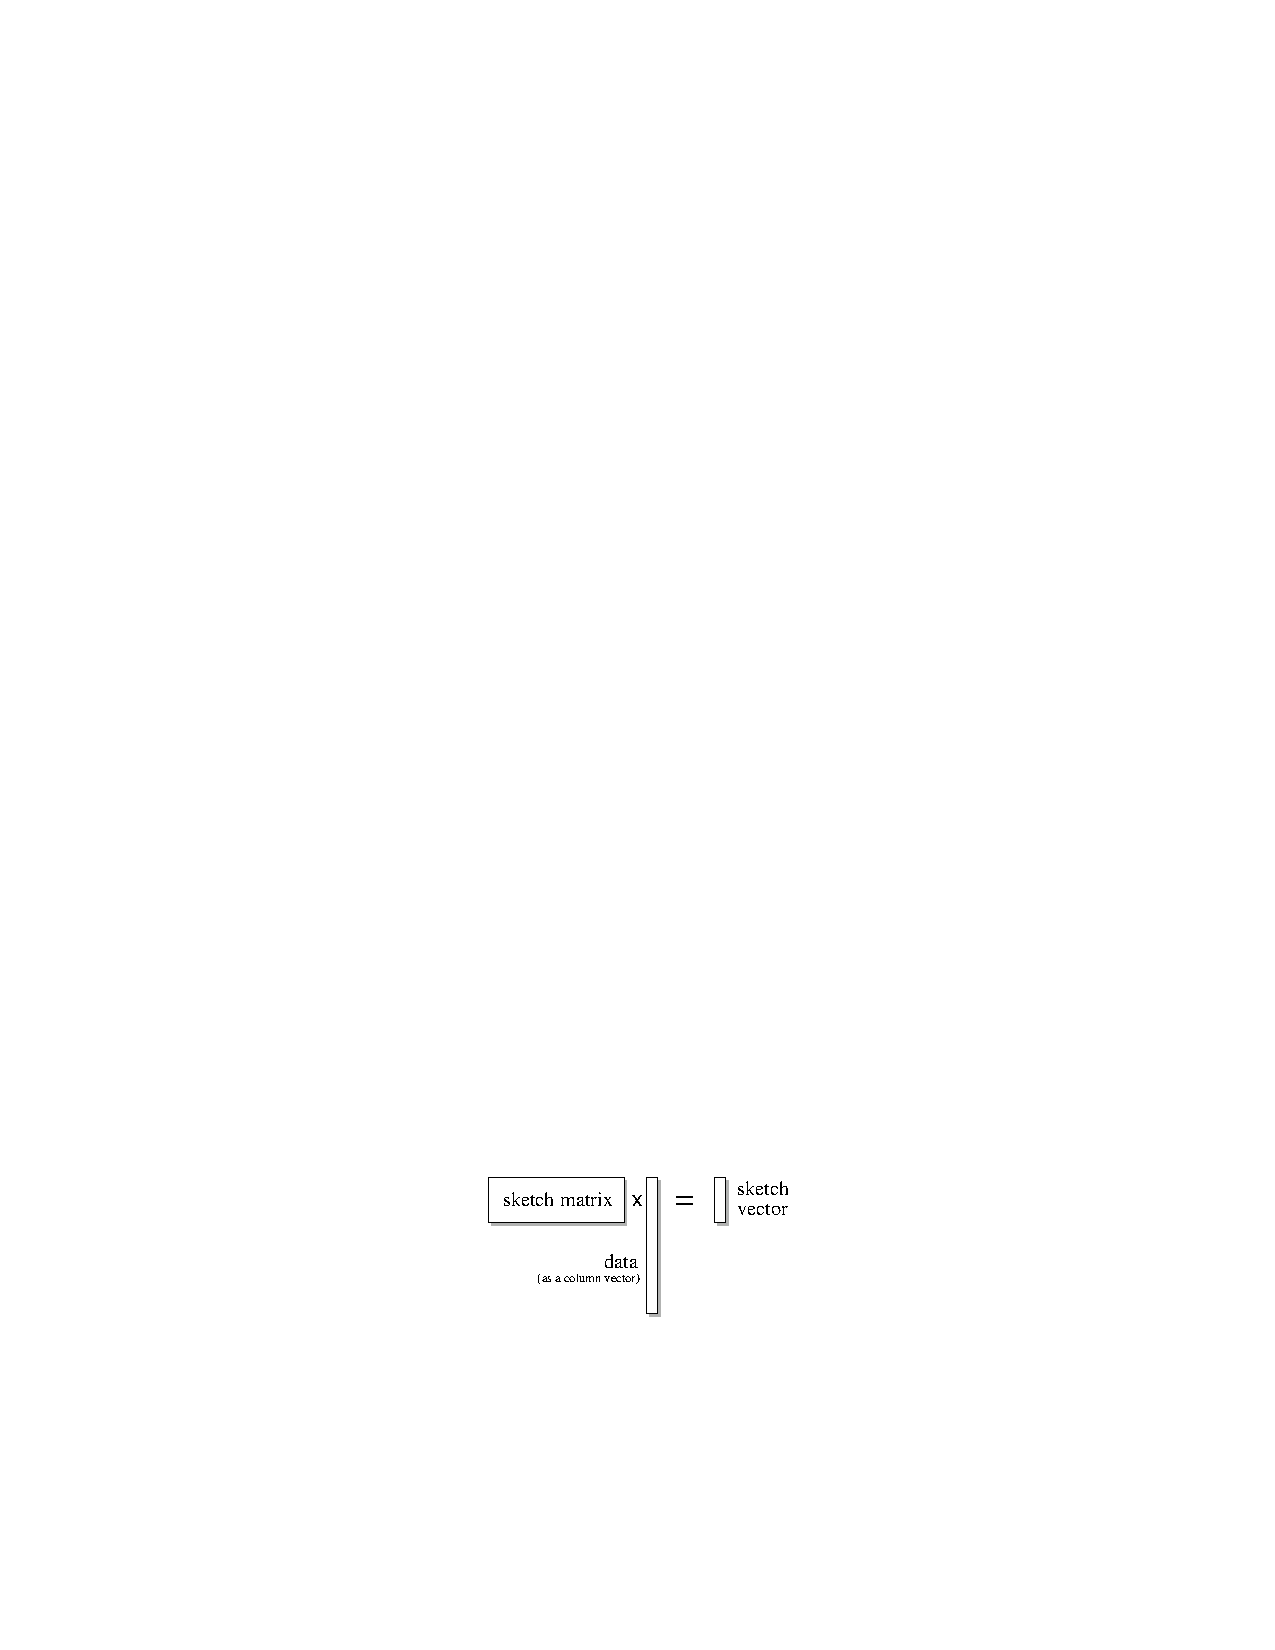
\includegraphics[width=0.5\textwidth]{linear-sketch-abstraction}
          \caption{Abstracción del \emph{Sketch Lineal}. \emph{(Extraida de \cite{cormode2012synopses})}}
          \label{fig:linear_sketch}
        \end{figure}

        \paragraph{}
        Puesto que la transformación que se muestra es de carácter lineal, entonces posee la propiedad de que siendo $S_1$ y $S_2$ dos \emph{Sketches} lineales, entonces se cumple la propiedad de que $S_1 + S_2 = S_{sum}$, lo que puede entenderse como la combinación de los estimadores de los dos \emph{Sketches}. Por tanto, se puede decir que el cada actualización se procesa como una transformación de la nueva instancia codificada en el vector $D$ para después combinar el \emph{Sketch} resultante con el generado anteriormente.

        \paragraph{}
        Por motivos de eficiencia a nivel de espacio, la matriz de transformación $A$ no se utiliza de manera explicita, sino que por contra, en muchos casos se utilizan distintas \emph{funciones hash} (las cuales se describen en la sección \ref{eq:hash_functions}), que realizan la transformación de la misma forma que la matriz $A$, solo que el coste computacional para utilizarlas es significativamente menor que el coste necesario para el almacenamiento y multiplicación de una matriz de tal tamaño.

        \paragraph{}
        Tal y como se puede apreciar en la figura \ref{fig:linear_sketch} la ventaja de sumarización de esta estrategia se obtiene en la reducción de tamaño obtenida en la transformación lineal. Posteriormente, cada estructura de \emph{Sketch} tiene asociadas un conjunto de \emph{consultas o queries} para las cuales extraer la información valiosa contenida en ellas. Puesto que la forma en que se llevan a cabo dichas consultas varía según la alternativa a la que nos estamos refiriendo, estas técnicas se expondrán en profundidad en sus correspondientes secciones.

        \paragraph{}
        Siguiendo con las restricciones descritas anteriormente, existe una implementación trivial de las estructuras de \emph{Sketch} consistente en mantener una tabla de frecuencias sobre cada posible instancia de entrada de tal manera que a partir de esta pueden resolver consultas como sumas de frecuencias, conteo de elementos distintos, búsqueda del máximo o mínimo, media o varianza del conjunto de datos. Sin embargo, esta solución no proporciona ninguna ventaja a nivel de espacio, por tanto, la tarea es encontrar técnicas que permitan \say{colapsar} dicha tabla de frecuencias para tratar de minimizar dicho coste asumiendo un cierto grado de imprecisión.

        \paragraph{}
        Existen dos categorías principales según la naturaleza de las consultas que el \emph{Sketch} puede responder. Dichas categorías se describen a continuación:

        \begin{itemize}

          \item \textbf{Estimación de Frecuencias}: Los \emph{Sketches} basados en estimación de frecuencias se corresponden con aquellos que tratan de recoger estimadores que se aproximen a la frecuencia de cada elementos $f(i)$. En esta categoría se enmarcan el \emph{Count-Min Sketch}, \emph{Count Sketch} y  \emph{AMS Sketch}.

          \item \textbf{Elementos Distintos}: Los \emph{Sketches} basados en el conteo de elementos distintos (y que también pueden responder consultas referidas a la presencia de un determinado elemento) se basan en el mantenimiento de distintos indicadores que permiten aproximar dichos valores. Entre los más destacados en esta categoría se encuentran el \emph{Bloom Filter} y el \emph{HyperLogLog}.

        \end{itemize}

        \paragraph{}
        A pesar de que todos los \emph{Sketches} siguen una estructura básica similar, existen distintos parámetros diferenciadores que caracterizan unas alternativas frente a otras entre las que destacan las consultas soportadas, el tamaño de los mismos (algunos necesitan menor espacio para obtener un grado de precisión similar a otros), el tiempo de procesamiento de cada nueva actualización (el cual se pretende que sea muy reducido debido al modelo en streaming), el tiempo de resolución de consultas o la estrategia de inicialización del mismo.


        \paragraph{}
        La extensión de los \emph{Sketches} sobre conjuntos de datos de caracter multidimensional puede resolverse utilizando funciones hash que mapeen una entrada multidimensional sobre un espacio unidimensional para después utilizarlos de la manera que para los casos de una dimensión. Esta solución no presenta problemas en la estimación de frecuencias puntuales o búsqueda de máximos o mínimos, sin embargo, no es factible para consultas de sumas de rangos utilizando \emph{sketches} multidimensionales o asumiendo la independencia entre dimensiones y manteniendo una estructura de \emph{sketch} por cada dimensión.

        \paragraph{}
        Los \emph{Sketches} presentan un gran nivel de simplicidad en sus implementaciones, lo que les hace muy eficientes y válidos para modelos que requieren de actualizaciones constantes como el descrito en el modelo en streaming. La dificultad de los mismos se basa en los conceptos matemáticos subyacentes, que complica en gran medida la demostración de sus características de convergencia hacia el valor real que estiman. Generalmente para reducir su espacio se apoyan en la utilización de funciones hash con distintas propiedades, pero que también se pueden calcular eficientemente. La mayor limitación se refiere al rango de consultas que cada tipo de \emph{Sketch} puede resolver de manera eficiente, estando especialmente limitados en el ámbito de múltiples consultas anidadas.

        \paragraph{}
        Los \emph{Sketches} son un ámbito interesante dentro del mundo de la investigación, con una visión de futuro muy prometedora que les coloca como la mejor solución a medio-largo plazo para la tarea del \emph{procesamiento de consultas aproximadas} por su reducido coste computacional, tanto a nivel de espacio como de tiempo de procesamiento. Actualmente universidades prestigiosas como la \emph{Universidad de California, Berkeley} o el \emph{MIT} están trabajando en el diseño de bases de datos que se apoyan fuertemente en el uso de estas estructuras. Dicha universidad está trabajando en una base de datos a la cual denominan \emph{BlinkDB} y la cual describen en el artículo \emph{BlinkDB: queries with bounded errors and bounded response times on very large data} \cite{agarwal2013blinkdb}

    \paragraph{}
    En las siguientes secciones se describen en profundidad distintas estructuras de datos basadas en \emph{Sketches} tratando de prestar especial importancia en una visión conceptual de la misma pero sin dejar de lado la parte práctica de las mismas. Además, se trata de incluir demostraciones acerca de la precisión de las mismas respecto del espacio utilizado para su almacenamiento respecto del tamaño del conjunto de datos global.


    \section{Bloom Filter}
    \label{sec:bloom_filter}

      \paragraph{}
      El \emph{Bloom-Filter} se corresponde con la primera estructura de datos basada en la idea de \emph{Sketch} por procesar cada nueva entrada de la misma forma y tener un coste a nivel de espacio sublineal ($o(N)$) respecto del cardinal de posibles valores que pueden ser procesados. Esta estructura de datos fue diseñada incialmente por \emph{Burton Howard Bloom} la cual describe en el artículo \emph{Space/time trade-offs in hash coding with allowable errors} \cite{bloom1970space} publicado en 1970.

      \paragraph{}
      La funcionalidad que suministra dicha estructura de datos es la consulta acerca de presencia de un determinado elemento. Para la implementación descrita en el artículo inicial no se permiten incrementos ni eliminaciones, tan solo la existencia o inexistencia del elemento, por tanto esta estructura de datos se enmar en el marco de \emph{serie temporal} del \emph{modelo en streaming}. El \emph{Bloom-Filter} asegura la inexistencia de falsos negativos (elementos que se presupone que no han sido introducidos cuando en realidad si que lo fueron) pero por contra, se admite una determinada tasa de falsos positivos (elementos que se presupone que han sido introducidos cuando en realidad no lo fueron).

      \paragraph{}
      Debido al tiempo de vida de dicha estrategia, su uso está muy asentado y se utiliza en distintos sistemas para tareas en las cuales se pretende optimizar el tiempo, pero sin embargo son admisibles fallos. Es comúnmente utilizado en bases de datos comerciales para limitar el número de accesos al disco durante búsquedas de elementos. Esto se lleva a cabo manteniendo un \emph{Bloom-Filter} al cual se consulta sobre la presencia del elemento a buscar y en el caso de que la respuesta sea negativa, entonces se prescinde de dicho acceso a la unidad de almacenamiento. Mientras que si es positiva se realiza el acceso a disco. Nótese por tanto que en algunos ocasiones dicho acceso será innecesario, sin embargo las consecuencias de dicha tarea tan solo tienen consecuencias negativas a nivel de eficiencia y no de resultados.

      \paragraph{}
      Una vez descrita la funcionalidad que proporciona el \emph{Bloom-Filter} así como un caso práctico de uso del mismo ya se tiene una idea a grandes rasgo acerca del mismo. Por tanto, lo siguiente es describir su composición. La estructura de datos se basa en el mantenimiento de un \emph{mapa de bits} $S$ de longitud $n$ ($|S| = n$) de tal manera que se cumpla que $n \ll m$ siendo $m$ el cardinal de elementos distintos que se pueden presentar en la entrada. Además, se utilizan $k$ funciones hash denominadas $h_1, h_2,..., h_j,..., h_k$ que distribuyen de manera independiente el elemento $i$-ésimo en $S$. El mapa de bits $S$ se inicializa con todas sus posiciones tomando el valor $0$.

      \paragraph{}
      El modo de funcionamiento del \emph{Bloom-Filter} se lleva a cabo de la siguiente manera: Cada vez que se presenta un nuevo elemento en la entrada (al cual denominaremos $i \in [1, m]$) se tomaran los $k$ valores de las funciones funciones hash indicadas anteriormente y se asignará el valor $1$ a dichas posiciones del mapa de bits $S$. Es decir, se realiza la operación descrita en la ecuación \eqref{eq:bloom_filter_update}. La consulta acerca de la presencia del elemento i-ésimo se realiza por tanto, consultando dichas posiciones, de tal manera que si $\forall j \in [1,k], \ S[h_j(i)]$ toma el valor valor $1$ se dice que el elemento ha aparecido en la entrada mientras que si alguna posición es distina de $1$ (toma el valor $0$) se dice que el elemento no ha sido introducido.

      \begin{equation}
      \label{eq:bloom_filter_update}
        \forall j \in [1,k], \ S[h_j(i)] = 1
      \end{equation}

      \paragraph{}
      Nótese que la restricción acerca de la presencia de un determinado elemento es mucho más débil que la de no existencia. La razón de ello se debe a que pueden existir colisiones entre las distintas funciones hash que conviertan dicho resultado en érroneo. Sin embargo, tal y como se ha indicado anteriormente, en caso de que el \emph{Bloom-Filter} indique la no presencia del elemento dicha respuesta será válida. A continuación se realiza un análisis acerca del índice de error para el caso de los falsos positivos la cual se basa en el artículo \emph{Network applications of bloom filters: A survey} \cite{broder2004network} de \emph{Broder} y \emph{Mitzenmacher}. Nótese que dicho análisis depende de 3 parámtros: el tamaño $n$ del mapa de bits, el cardinal $m$ del conjunto de posibles elementos en la entrada y el número $k$ de funciones hash utilizadas.

      \begin{figure}
        \centering
        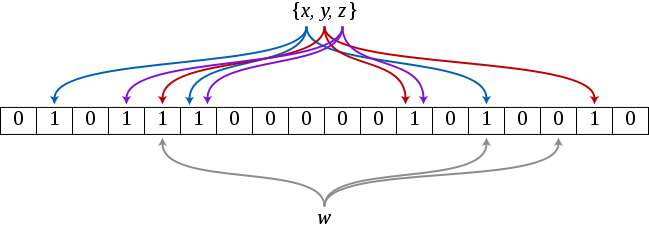
\includegraphics[width=0.5\textwidth]{bloom-filter}
        \caption{Modo de funcionamiento del \emph{Bloom Filter}, que inserta los valores $\{ x, y, z\}$ y comprueba la existencia de $w$. La imagen ha sido extraida de \cite{wiki:Bloom_filter}.}
        \label{fig:bloom_filter}
      \end{figure}

      \paragraph{}
      Para el análisis se presupone que las funciones hash $h_j$ son totalmente aleatorias, es decir, distribuyen los valores de manera totalmente uniforme en el intervalo $[1,n]$ y son totalmente independientes entre sí. La probabilidad $p'$ de que cualquier posición de $S$ siga siendo igual a cero después de la aparición de $l$ elementos distintos se muestra en la ecuación \eqref{eq:bloom_filter_p_estimator} siendo la base del lado derecho de la igualdad la probabilidad de que cada función hash mantenga con el valor $0$ una posición.

      \begin{equation}
      \label{eq:bloom_filter_p_estimator}
       p' = \bigg(1-\frac{1}{m}\bigg)^{kl}
      \end{equation}

      \paragraph{}
      La probabilidad de que un elemento no introducido en la entrada tome todas sus correspondientes posiciones de $S$ con el valor $1$ se da con probabilidad $(1-p)^k$ y dado que $p'$ es un buen estimador para $p$, entonces podemos aproximar la tasa de falsos positivos. Tras desarrollar dicha expresión se puede llegar a la ecuación \eqref{eq:bloom_filters_false_positives}, que aproxima de manera apropiada la tasa de falsos positivos.

      \begin{equation}
      \label{eq:bloom_filters_false_positives}
        f = (1-e^{-kn/m})^k
      \end{equation}

      \paragraph{}
      El \emph{Bloom-Filter} es una buena aproximación para los casos en que es necesario reducir el sobre coste de comprobación de accesos a medios costosos, sin embargo, su utilización puede utilizarse en filtros anti-spam u otros entornos en que una determinada tasa de error sea admisible. Nótese que este típo de \emph{Sketches} no puede agruparse en el subconjunto de \emph{Sketches Lineales} puesto que la operación de asignar el valor $1$ no es lineal.

    \section{Count-Min Sketch}
    \label{sec:count_min_sketch}

      \paragraph{}
      El \emph{Count-Min Sketch} es otra estructura de datos con la característica de presentar un coste espacial de carácter sublineal ($o(N)$) respecto del cardinal de posibles elementos de entrada. El \emph{Count-Min Sketch} (en adelante \emph{CM Sketch} por abreviación) fue descrito por primera vez por \emph{Cormode} y \emph{Muthukrishnan} en el artículo \emph{An improved data stream summary: the count-min sketch and its applications} \cite{cormode2005improved} publicado en 2005. Nótese por tanto que el tiempo de vida de dicha estructura de datos es muy corto.

      \paragraph{}
      El propósito del \emph{CM Sketch} es la estimación de frecuencias para el rango de posibles valores que se presentan en la entrada. En la formulación inicial se enmarcaba modelo de caja registradora, que tan solo permite adicciones, sin embargo posteriormente se han propuesto mejoras para ampliar su uso en entornos en que también se permitan eliminaciones (modelo en molinete). Tal y como se verá a continuación, el nombre de este \emph{Sketch} se refiere a las operaciones de operaciones que utiliza durante su funcionamiento, es decir, el conteo o suma y la búsqueda del mínimo.

      \paragraph{}
      La estimación de frecuencias del \emph{CM Sketch}, tal y como se puede apreciar debido al carácter sublineal del mismo, no garantiza la exactitud en de los mismos, sino que al igual que en el caso del \emph{Bloom-Filter} devuelve como resultado una aproximación. En este caso dicha aproximación garantiza que el resultado estimado siempre será mayor o igual que el verdadero, es decir, realiza una sobre-estimación del valor real. La razón por la cual el \emph{CM Sketch} utiliza la operación de búsqueda del mínimo es para tratar de reducir dicho efecto en la medida de lo posible.

      \paragraph{}
      Debido al corto periodo de vida su uso todavía no está asentado en sistemas reales, sin embargo existen una gran variedad de situaciones que se enmarcan sobre el modelo en streaming en las cuales la precisión de frecuencias no tienen grandes efectos perjudiciales. Un ejemplo de ello podría ser el conteo de visitas a un determinado sitio web formado por distintas páginas. La estimación sobre el número de visitas para cada una de estas páginas podría llevarse a cabo utilizando esta estructura de datos, ya que es una tarea que puede admitir una determinada tasa de error y requiere de actualizaciones constantes.

      \paragraph{}
      Una vez descrita la funcionalidad que suministra el \emph{CM Sketch} se describirá la estructura interna del mismo: Esta estructura de datos está formada por una matriz $S$ de estructura bidimensional con $w$ columnas y $d$ filas, de tal manera que se mantienen $w * d$ contadores. Cada una de las $d$ filas tiene asociada una función hash $h_j$ que distribuye elementos pertenecientes al dominio $[1, m]$ (siendo $m$ el cardinal de elementos distintos) sobre la fila de dicha matriz, es decir, sobre $[1,w]$. Para que las estimaciones acerca de la precisión del \emph{CM Sketch} sean correctas cada función hash $h_j$ debe cumplir la propiedad de ser independiente del resto además de seguir una distribución uniforme. En cuanto a la inicialización de la estructura de datos, todas las posiciones toman el valor cero, esto se muestra en la ecuación \eqref{eq:count_min_sketch_init}.

      \begin{equation}
      \label{eq:count_min_sketch_init}
        \forall k \in [1,w], \ \forall j \in [1,d], \ S[k,j] = 0
      \end{equation}


      \paragraph{}
      En cuanto al modo de funcionamiento del \emph{CM Sketch}, tal y como se ha indicado anteriormente, se enmarca en el modelo de caja registradora, es decir, cada actualización se corresponde con una tupla formada por el identificador del elemento al que se refiere y un determinado valor positivo que indica el incremento $c$ al cual se refiere la actualización. El funcionamiento es similar al del \emph{Bloom-Filter} en el sentido de que por cada nueva entrada se realizan $d$ actualizaciones (una para cada fila). La operación de conteo se refiere a dicha actualización, que se ilustra de manera matemática en la ecuación \eqref{eq:count_min_sketch_update}. Una representación gráfica de dicha operación se muestra en la figura \ref{fig:count_min_sketch}. Nótese por tanto que el coste de actualización es de $O(d)$.

      \begin{equation}
      \label{eq:count_min_sketch_update}
        \forall j \in [1,d], \ S[j, h_j(i)] = S[j, h_j(i)] + c
      \end{equation}

      \paragraph{}
      En cuanto al proceso de consulta sobre la frecuencia del elemento i-ésimo, esto se lleva a cabo recogiendo el valor almacenado en cada fila y devolviendo el menor, de tal manera que se pretende reducir el efecto de las colisiones generados sobre las funciones hash al distribuir elementos sobre un espacio de menor tamaño, ya que se presupone que $w * d \ll m$ para que la ventaja a nivel de espacio se produzca. Dicha operación se muestra en la ecuación \eqref{eq:count_min_sketch_estimate}

      \begin{equation}
      \label{eq:count_min_sketch_estimate}
        \widetilde{f}(i) = min_{j \in [1,d]}\{S[j, h_j(i)]\}
      \end{equation}

      \paragraph{}
      A nivel de análisis acerca del coste espacial necesario para almacenar en memoria el \emph{CM Sketch} este es dependiente del grado de precisión que se pretenda asegurar mediante el uso del mismo. Sin embargo, el análisis no se realiza sobre el cardinal de posibles elementos que pueden aparecer en la entrada, sino que depende del sumatorio del conteo de los mismos. A este valor se le define como $N$ tal y como se indica en la ecuación \eqref{eq:count_min_sketch_sum}.

      \begin{equation}
      \label{eq:count_min_sketch_sum}
        N = \sum_{i=1}^m \widetilde{f}(i)
      \end{equation}

      \begin{figure}
        \centering
        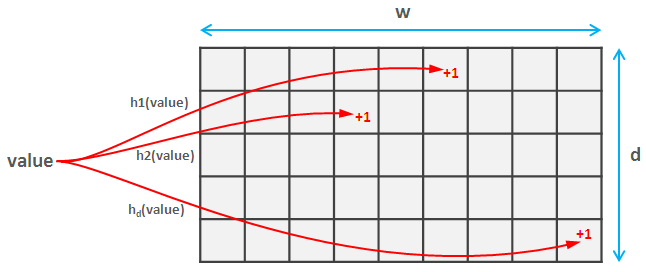
\includegraphics[width=0.5\textwidth]{count-min-sketch}
        \caption{Modo de funcionamiento del \emph{Count-Min Sketch} durante el proceso de inserción de un nuevo elemento. La imagen ha sido extraida de \cite{cormode2005improved}.}
        \label{fig:count_min_sketch}
      \end{figure}

      \paragraph{}
      Por tanto, la precisión de esta estructura de datos probabilística se indica diciendo que $\widetilde{f}(i)$ tendrá un error máximo de $\epsilon N$ que el cual se cumplirá con probabilidad $1-\delta$. Estos parámetros se fijan en el momento de la inicialización del \emph{CM Sketch} fijando el número de filas y columnas de tal manera que $d = log(1/\delta)$ y $w=2/\epsilon$. La demostración acerca de la elección de estos valores puede encontrarse en el artículo original \cite{cormode2005improved}.

      \paragraph{}
      En cuanto a la estimación de frecuencias obtenida por el \emph{CM Sketch}, en sentido estricto se dice que esta es sesgada respecto de su valor real. La razón se debe a que siempre se produce una sobre-estimación, a pesar de tratar de reducir los efectos negativos de la misma tratando de seleccionar el mínimo de las estimaciones siempre será mayor o igual (nunca menor). Para tratar de solventar esta problemática se han propuesto distintas heurísticas que tratan de contrarrestar esta problemática en el modelo de caja de registradora (tan solo se permiten inserciones).

      \paragraph{}
      Sin embargo, dicho problema no sucede en el caso del modelo general o de molinete, sobre el cual si que están permitidas las eliminaciones. En este caso es más apropiado utilizar como estimación la mediana de los valores almacenados en cada columna, puesto que se escoge el mínimo para un elemento que tan solo ha recibido actualizaciones negativas probablemente este será muy diferente del valor real. La razón por la cual se escoge la mediana y no la media es por sus propiedades de resistencia ante valor atípicos u \emph{outliers}. En este caso la demostración se puede llevar a cabo apoyandose en la desigualdad de Chernoff descrita en la sección \ref{sec:chernoff_inequality}. Esta demostración se puede encontrar en el artículo \emph{Selection and sorting with limited storage }\cite{munro1980selection} de \emph{Munro} y \emph{Paterson}.

      \paragraph{}
      El \emph{Count-Min Sketch} consiste en una estrategia apropiada para el conteo de ocurrencias en un espacio de orden sublineal. Además, la implementación del mismo es simple en contraposición con otras estrategias más sofisticadas. En posteriores secciones se hablará del \emph{Count Sketch} y el \emph{AMS Sketch}, que proporcionan valores de precisión equivalentes en espacios de menor tamaño añadiendo una mayor complejidad conceptual.


    \section{Count Sketch}
    \label{sec:count_sketch}

      \paragraph{}
      [TODO ] \emph{Finding frequent items in data streams} \cite{charikar2002finding}

    \section{AMS Sketch}
    \label{sec:ams_sketch}

      \paragraph{}
      [TODO ] \emph{The space complexity of approximating the frequency moments} \cite{alon1996space}

    \section{HyperLogLog}
    \label{sec:hyper_log_log}

      \paragraph{}
      [TODO ] \emph{Hyperloglog: the analysis of a near-optimal cardinality estimation algorithm} \cite{flajolet2007hyperloglog}


\end{document}
